\newpage
\section{Activity Diagram}

\subsection{Quản trị Hệ thống và Tích hợp}

\noindent \textbf{Đăng nhập}
\begin{figure}[H]
    \centering
    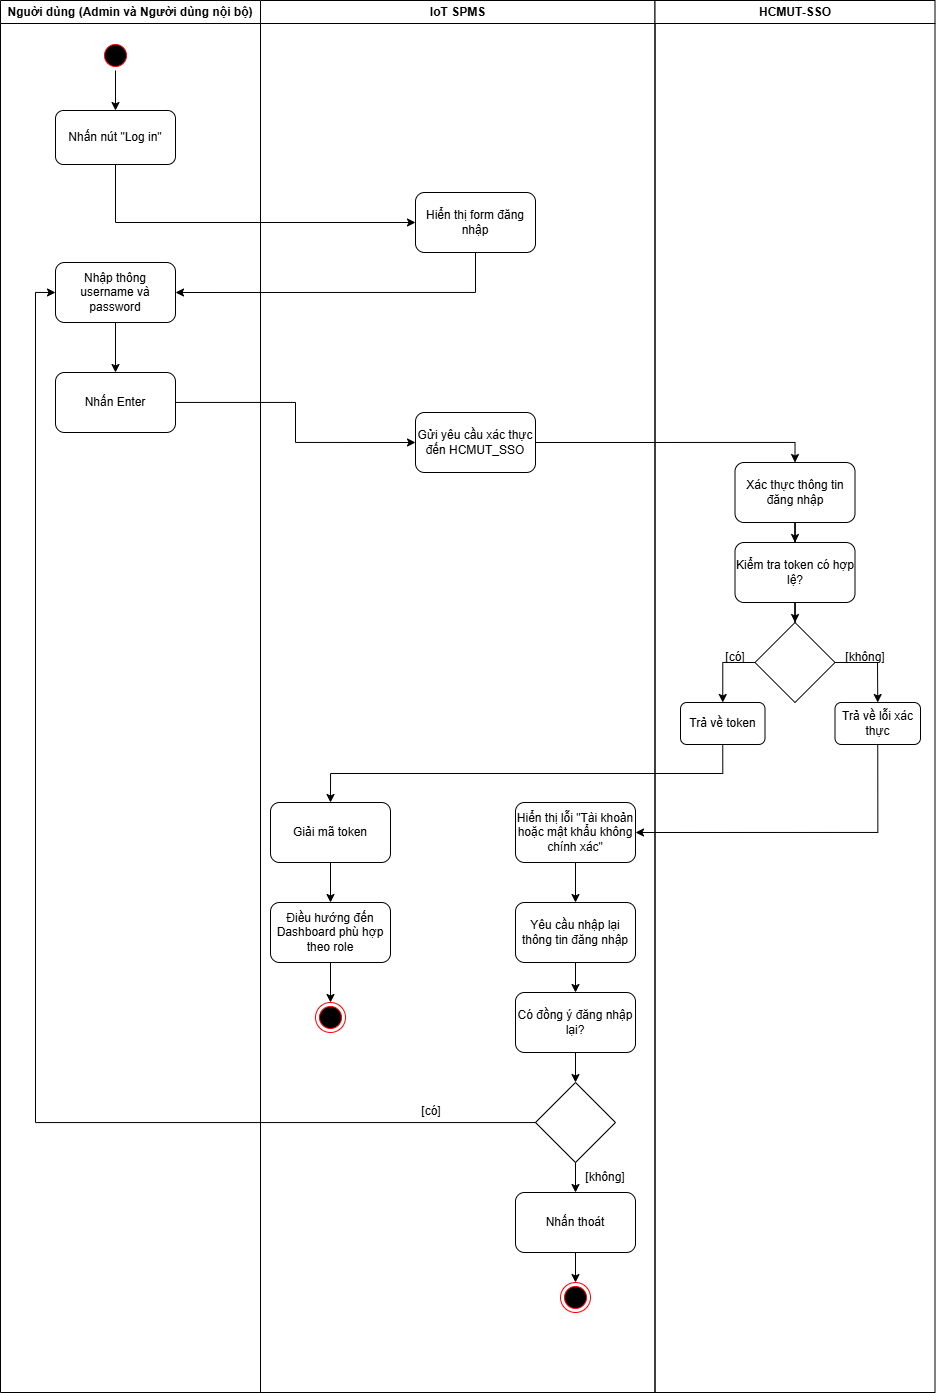
\includegraphics[width=0.8\textwidth]{pictures/act_diagram/login_act.drawio.png} 
    \caption{Activity Diagram cho use-case Đăng nhập}
    \label{login_act}
\end{figure}

\newpage
\noindent \textbf{Đồng bộ thông tin người dùng}
\begin{figure}[H]
    \centering
    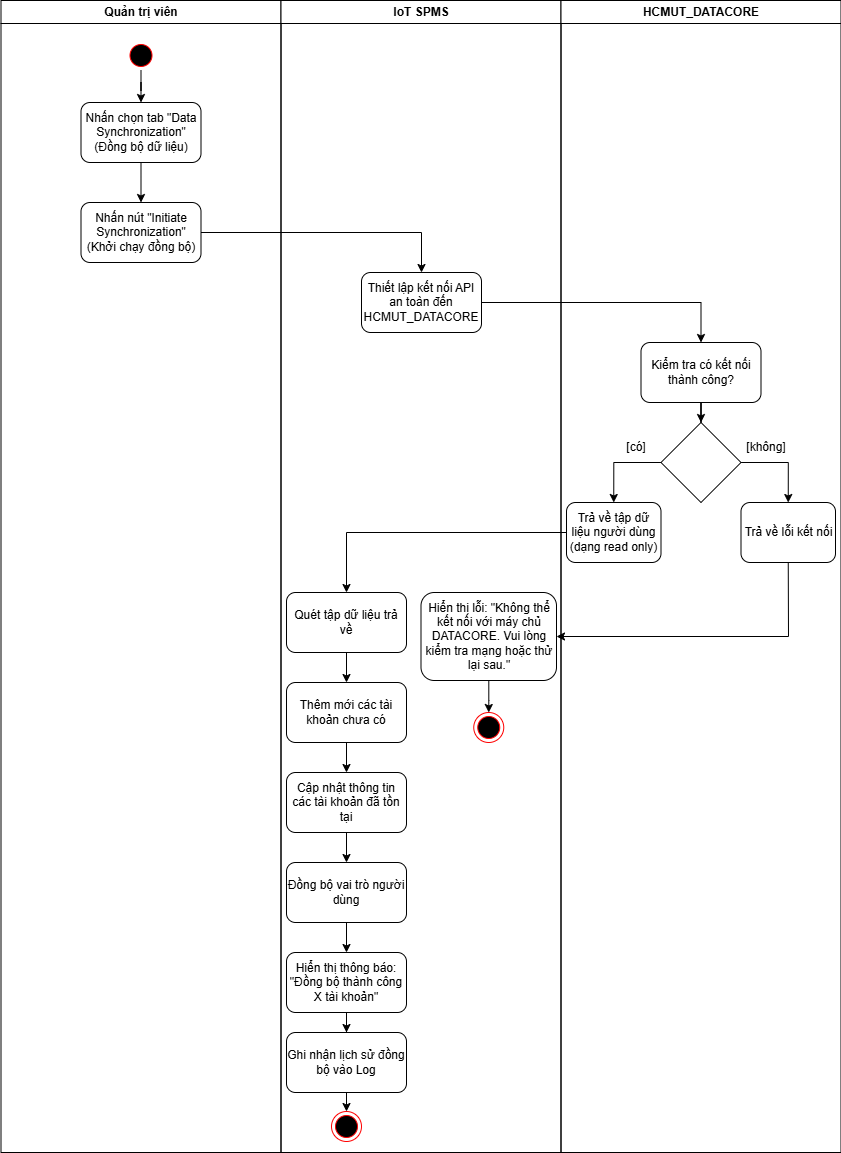
\includegraphics[width=0.8\textwidth]{pictures/act_diagram/sync_act.drawio.png} 
    \caption{Activity Diagram cho use-case Đồng bộ thông tin người dùng}
    \label{sync_act}
\end{figure}

\newpage
\noindent \textbf{Phân quyền người dùng}
\begin{figure}[H]
    \centering
    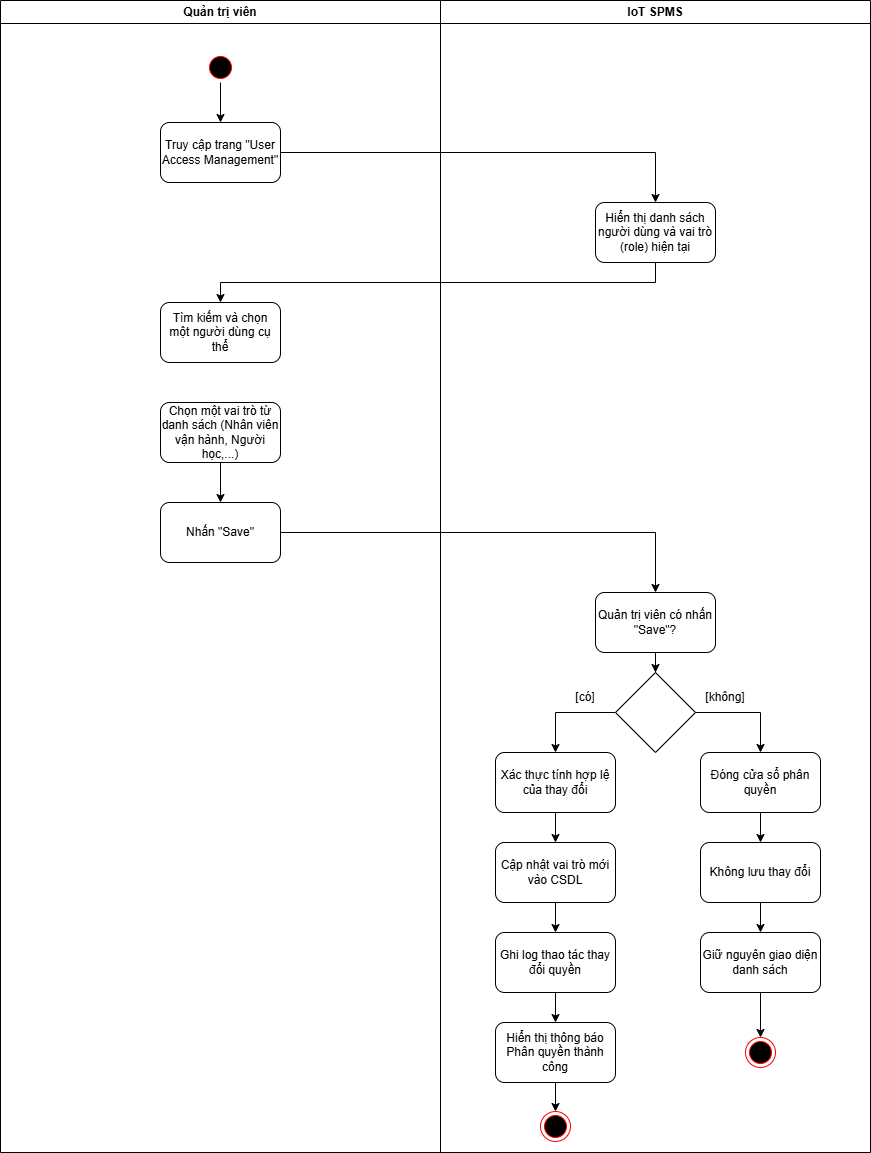
\includegraphics[width=0.8\textwidth]{pictures/act_diagram/useraccess_act.drawio.png} 
    \caption{Activity Diagram cho use-case Phân quyền người dùng}
    \label{user_act}
\end{figure}

%----------------------------------------------------------------------------
\subsection{Quản lý kiểm soát ra vào}

\noindent \textbf{Xe vào bãi bằng thẻ ID}
\begin{figure}[H]
    \centering
    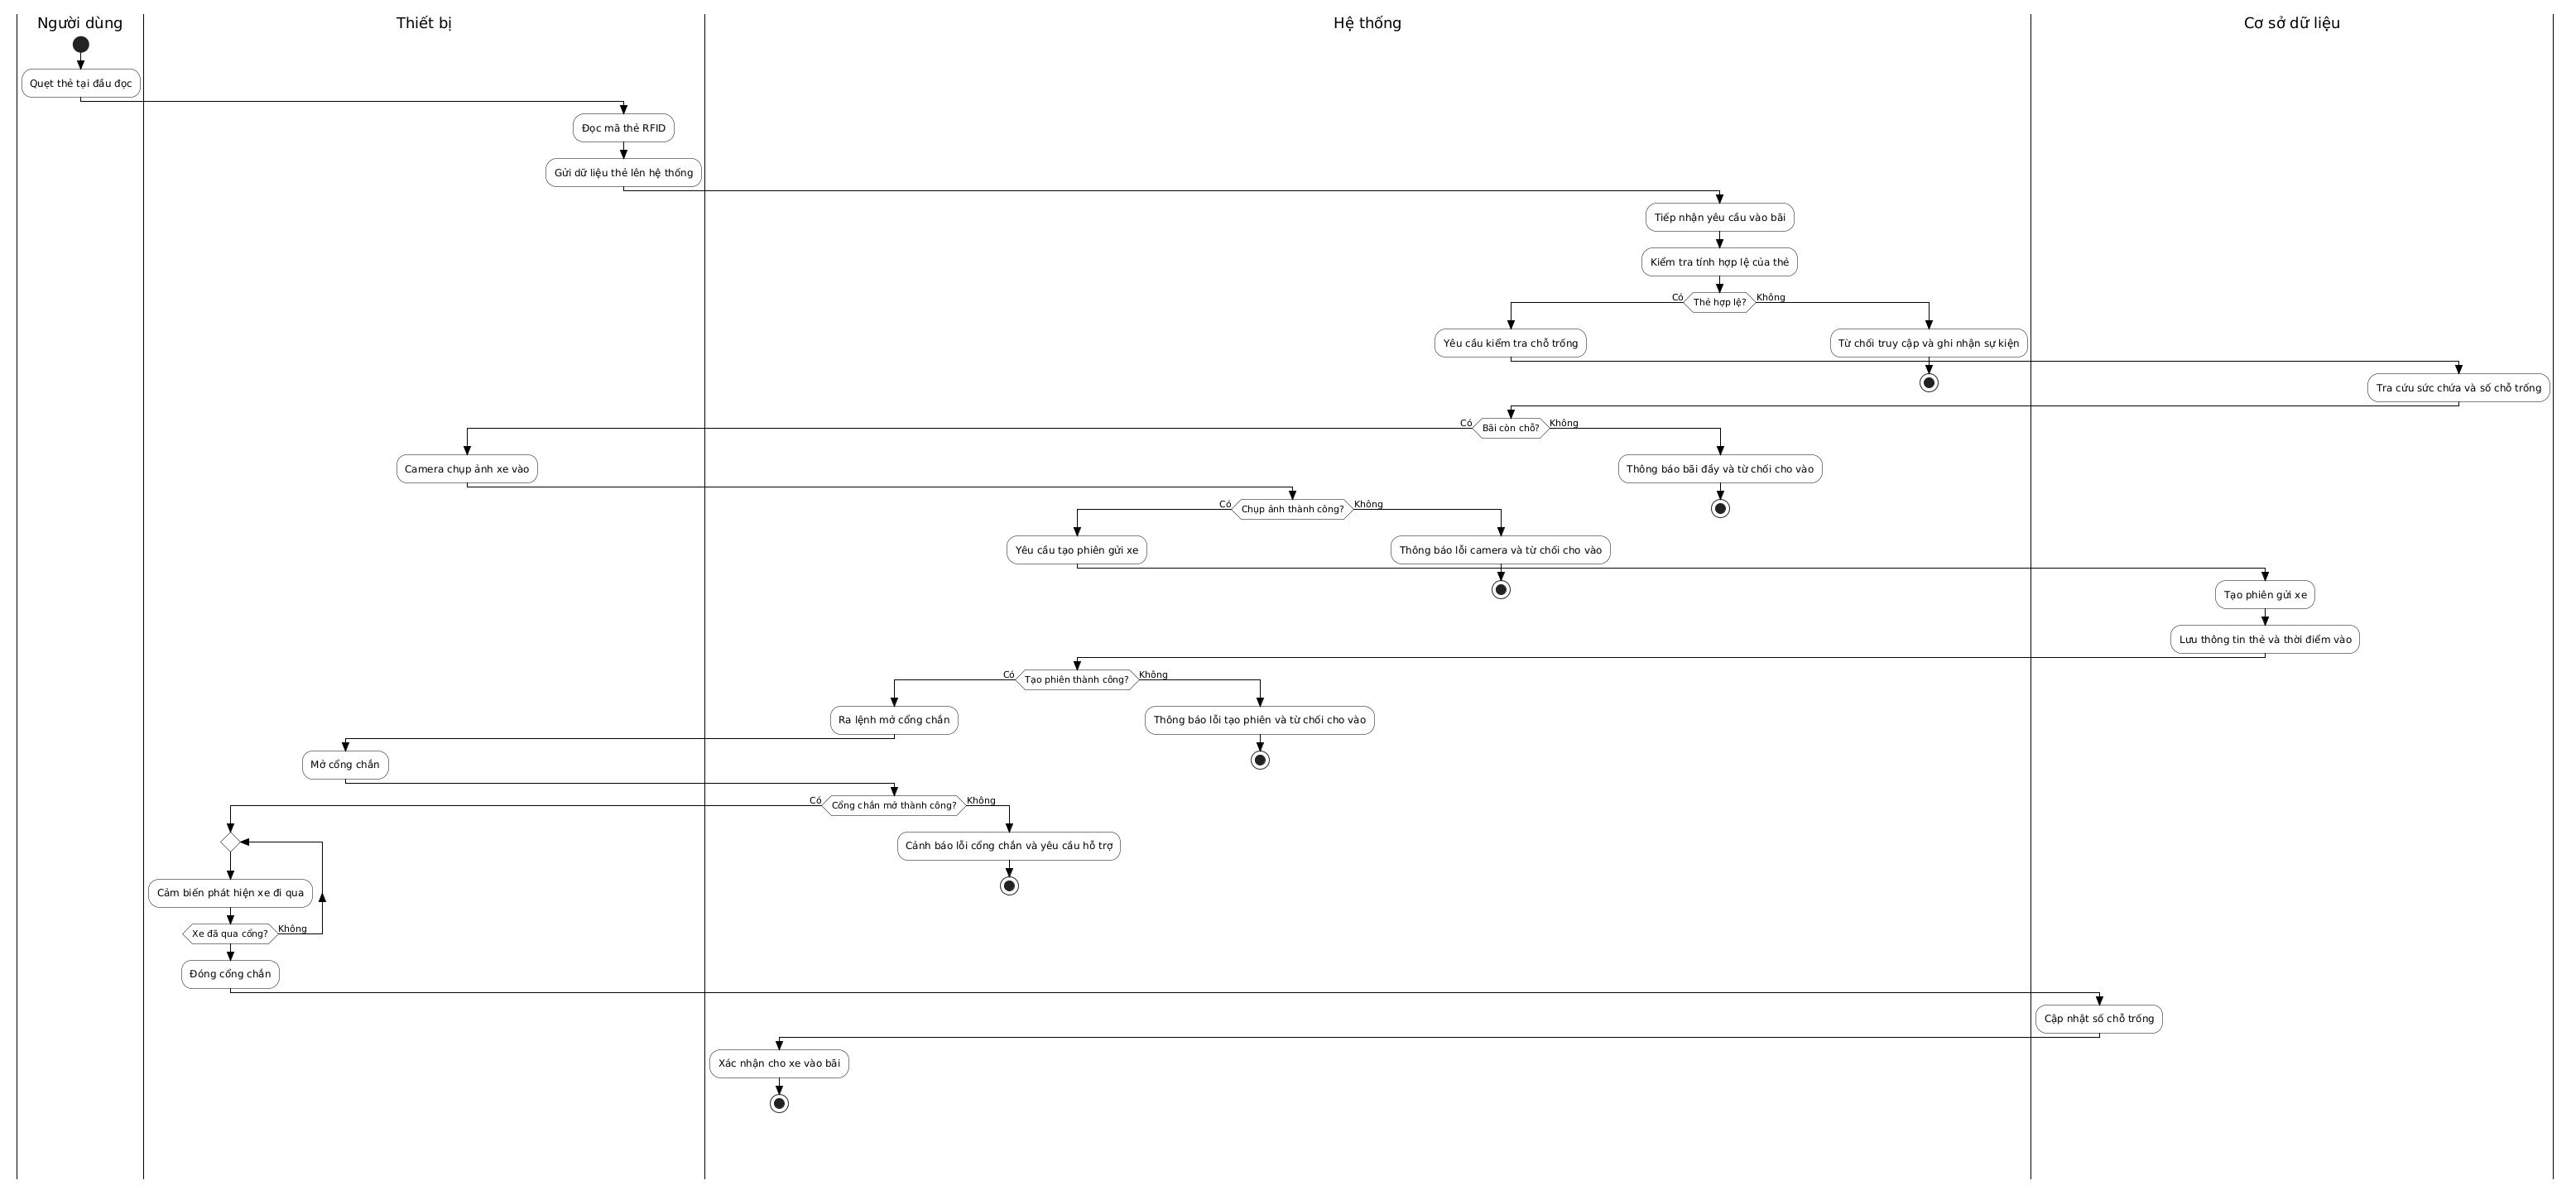
\includegraphics[width=0.8\textwidth]{pictures/act_diagram/enter_parking_act.png} 
    \caption{Activity Diagram cho use-case Vào bãi xe bằng thẻ ID}
    \label{enter_parking_act}
\end{figure}

\newpage
\noindent \textbf{Xe rời bãi bằng thẻ ID}
\begin{figure}[H]
    \centering
    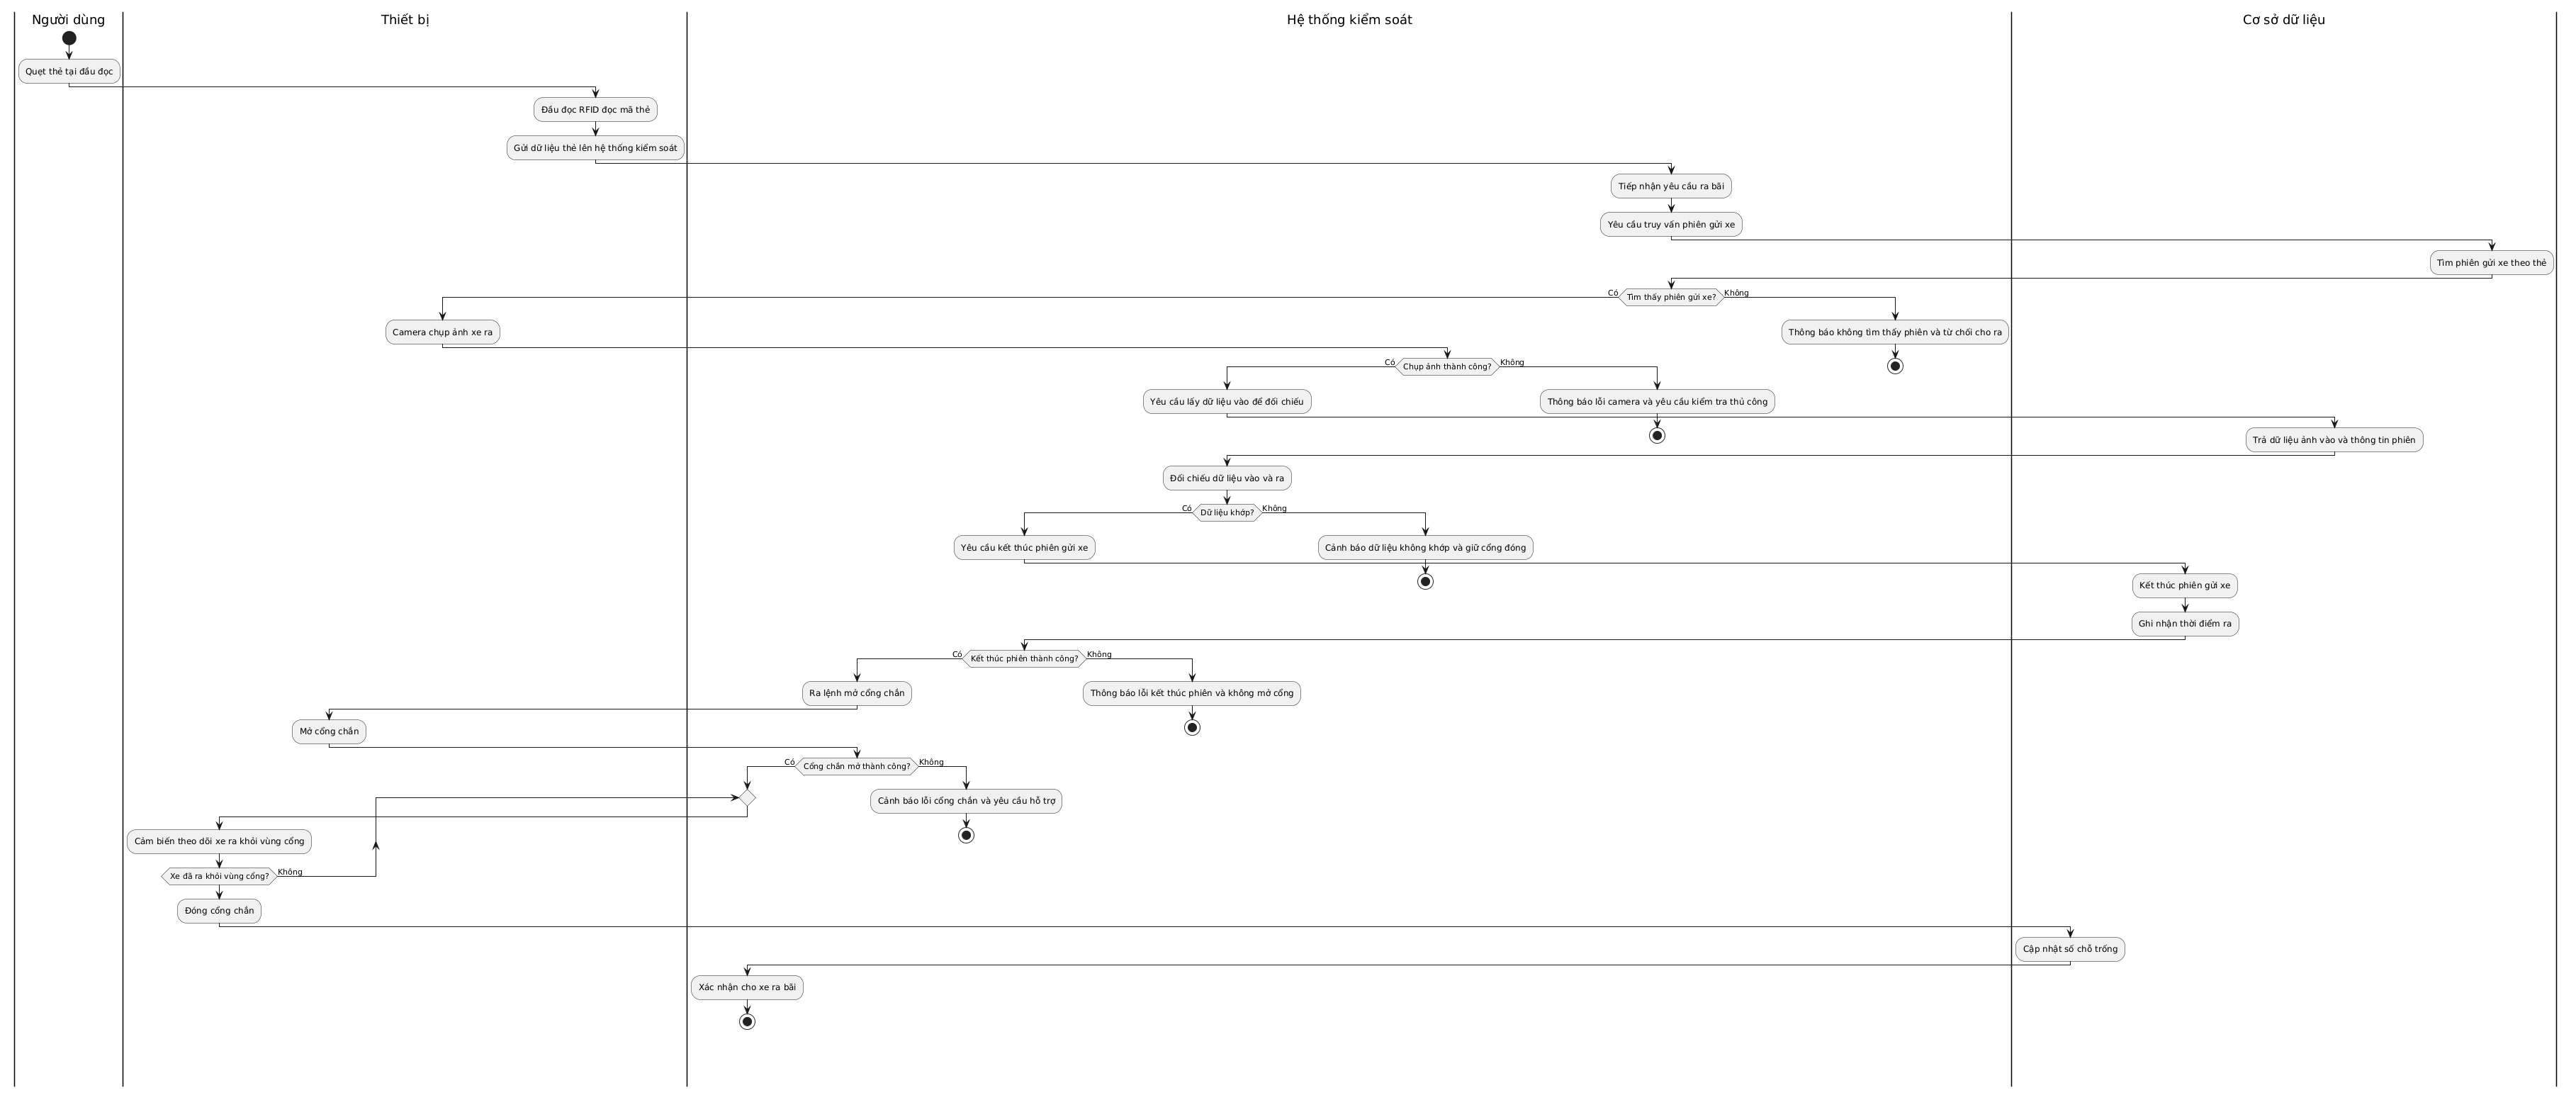
\includegraphics[width=0.8\textwidth]{pictures/act_diagram/exit_parking_act.png} 
    \caption{Activity Diagram cho use-case Rời bãi xe bằng thẻ ID}
    \label{exit_parking_act}
\end{figure}

\newpage
\noindent \textbf{Phát hành vé tạm thời}
\begin{figure}[H]
    \centering
    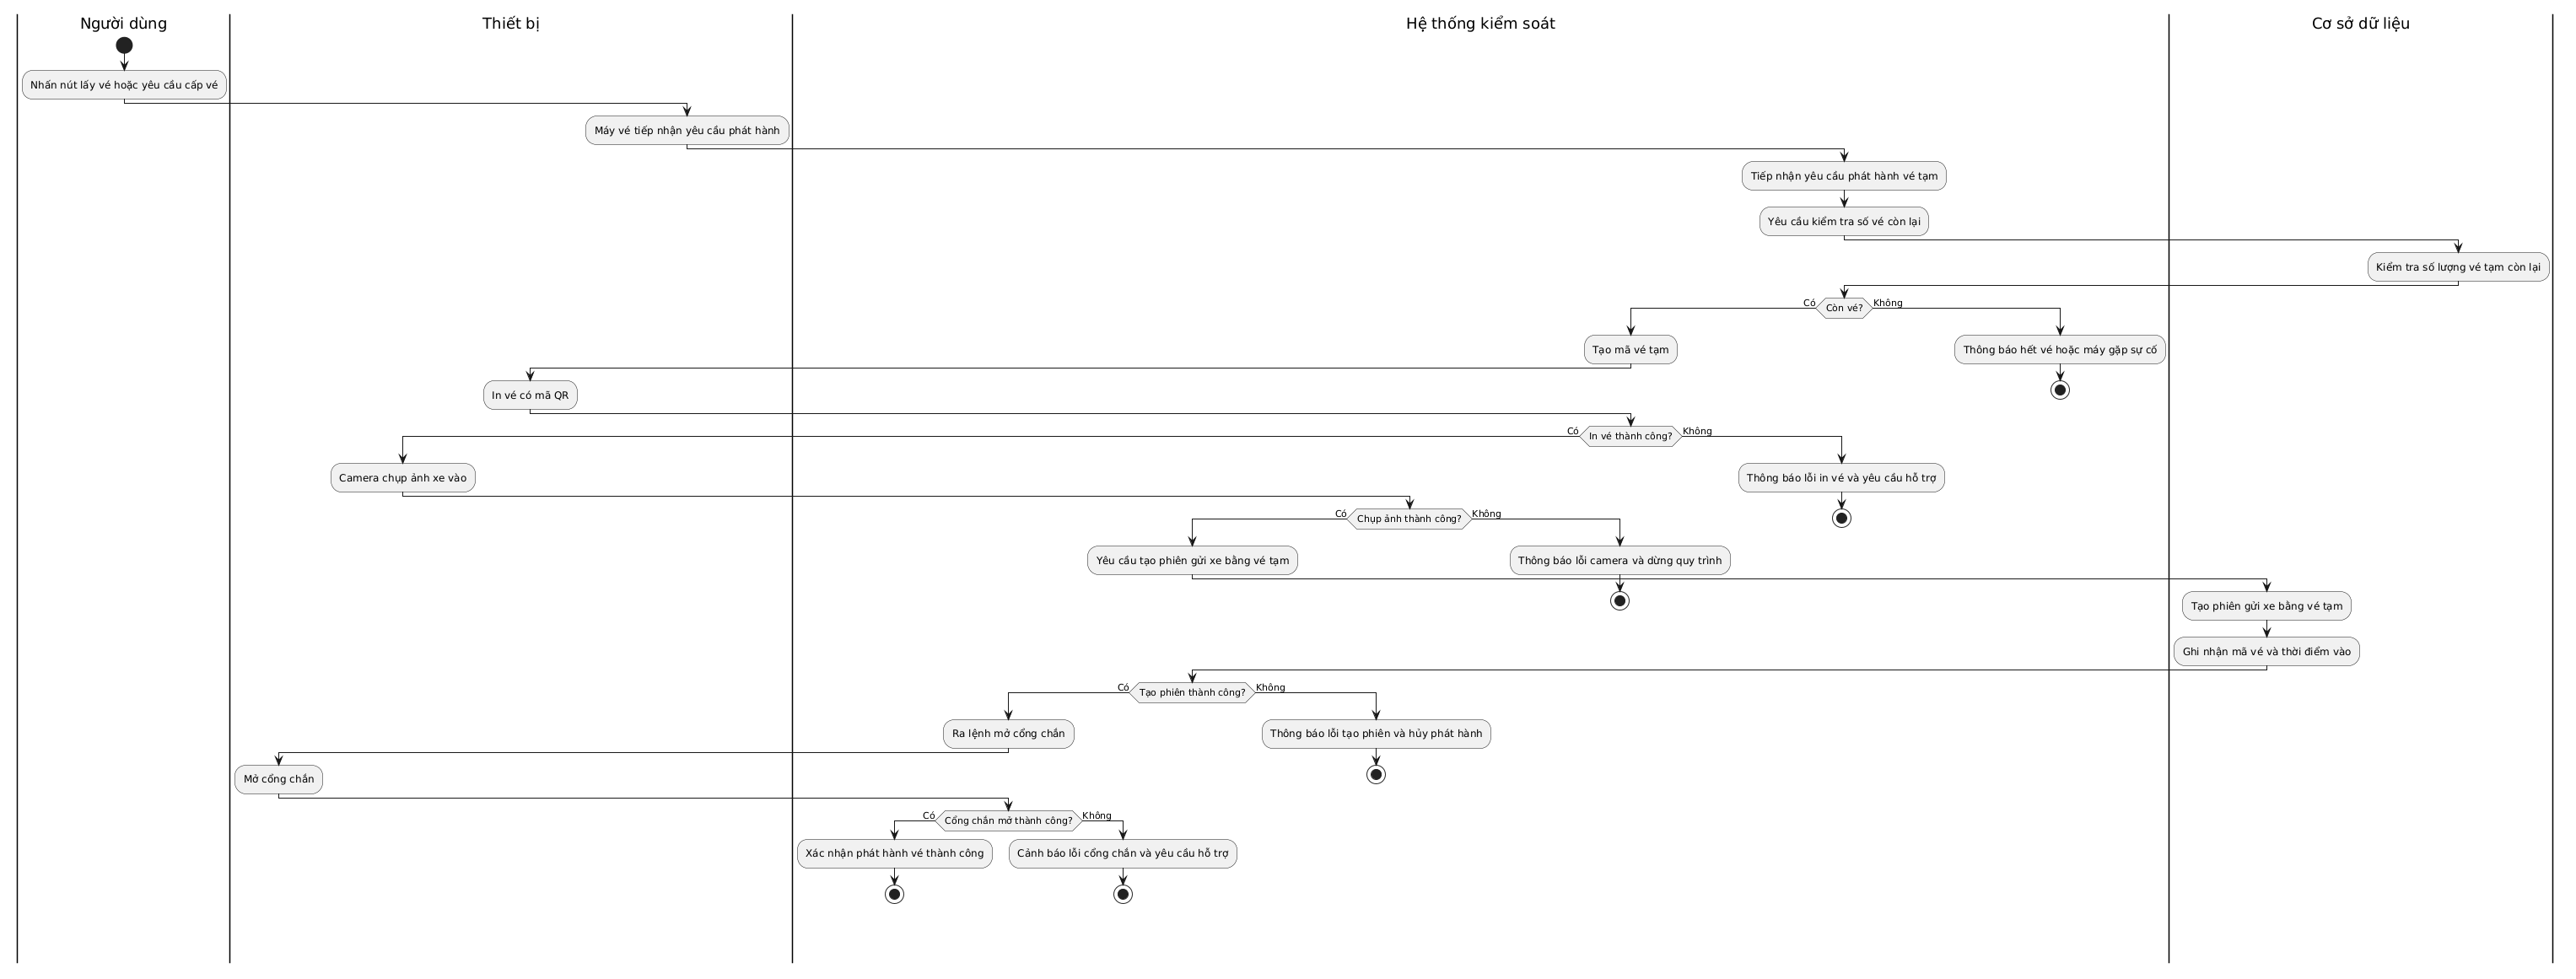
\includegraphics[width=0.8\textwidth]{pictures/act_diagram/temp_ticket_act.png} 
    \caption{Activity Diagram cho use-case Phát hành vé tạm thời}
    \label{temp_ticket_act}
\end{figure}

\newpage
\noindent \textbf{Quản lý phiên ngoại tuyến}
\begin{figure}[H]
    \centering
    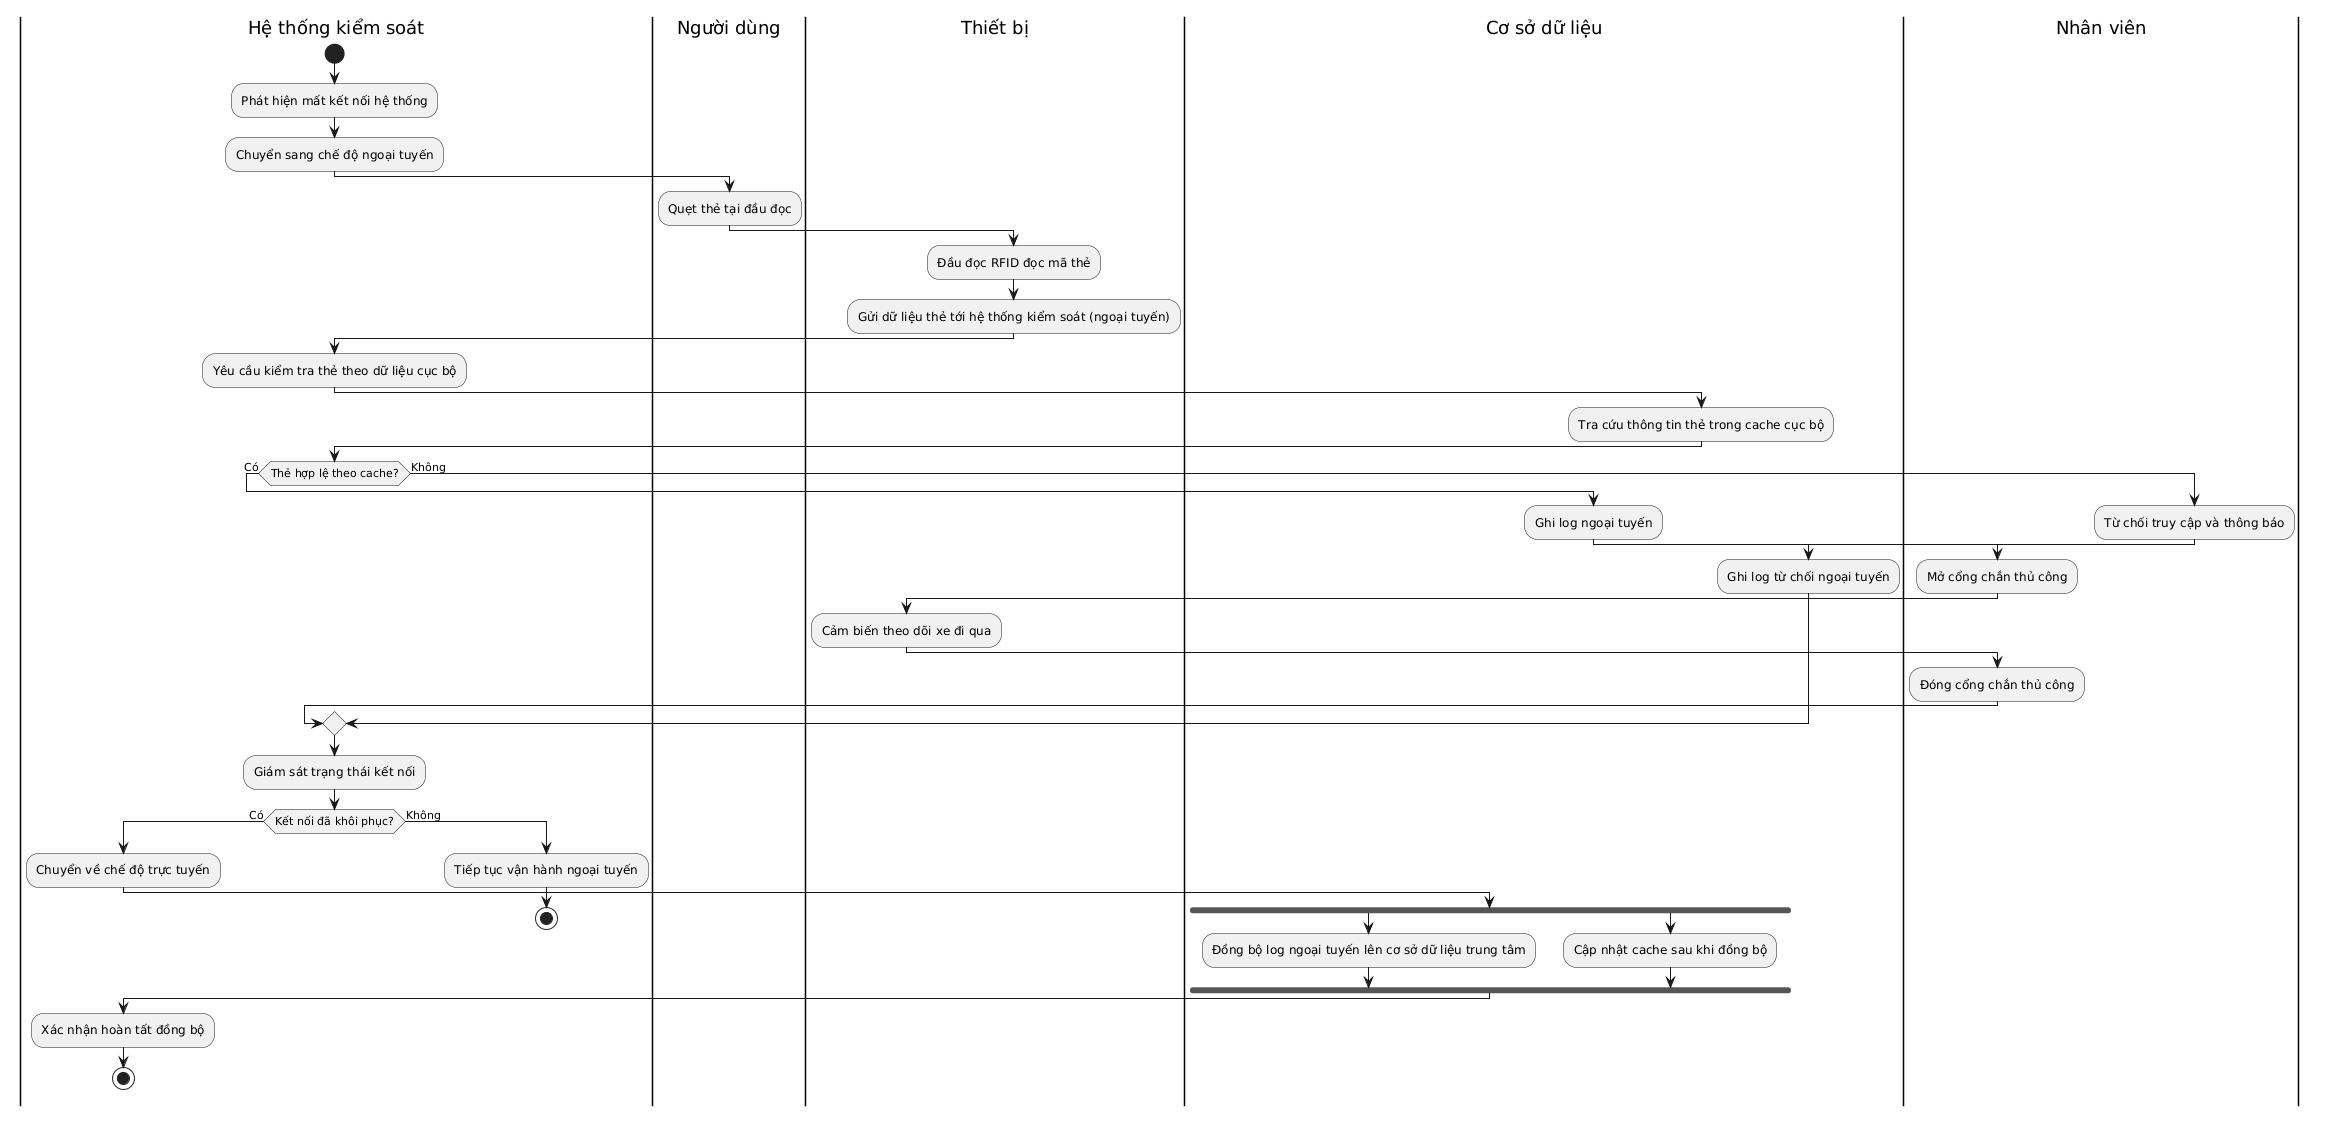
\includegraphics[alt={Mô tả chi tiết về hình ảnh của bạn},width=0.8\textwidth]{pictures/act_diagram/off_ctrl_act.png} 
    \caption{Activity Diagram cho use-case  Quản lý phiên ngoại tuyến}
    \label{off_control_act}
\end{figure}

%----------------------------------------------------------------------------
\subsection{Giám sát IOT và trạng thái bãi đỗ}
\noindent \textbf{xem sơ đồ bãi đỗ thời gian thực}
\begin{figure}[H]
    \centering
    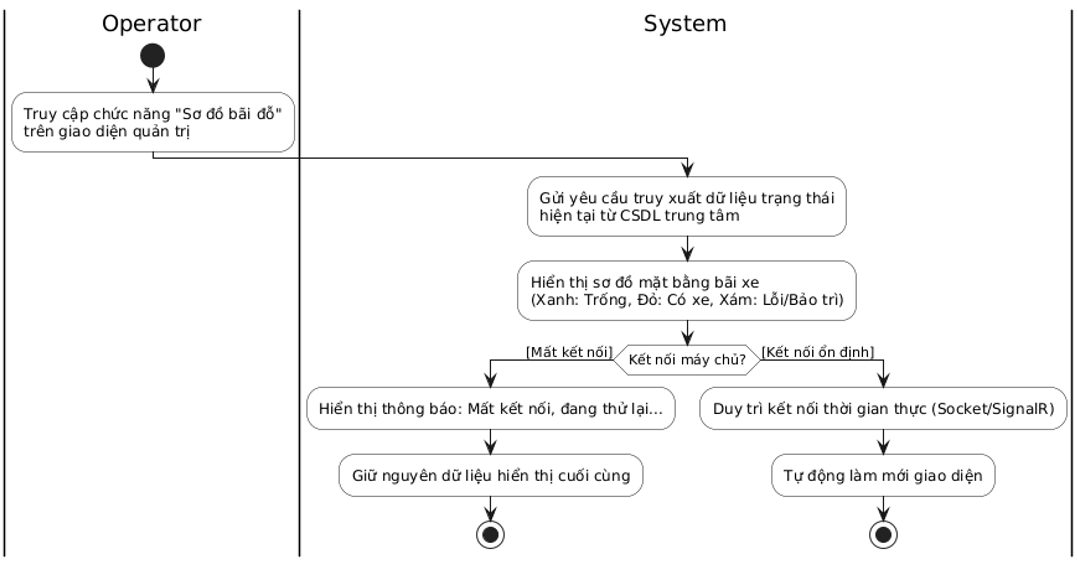
\includegraphics[width=0.8\textwidth]{pictures/act_diagram/ac_1.png} 
    \caption{Activity Diagram cho use-case Xem sơ đồ bãi đỗ thời gian thực}

\end{figure}

\newpage
\noindent \textbf{Tự động cập nhật trạng thái ô đỗ}
\begin{figure}[H]
    \centering
    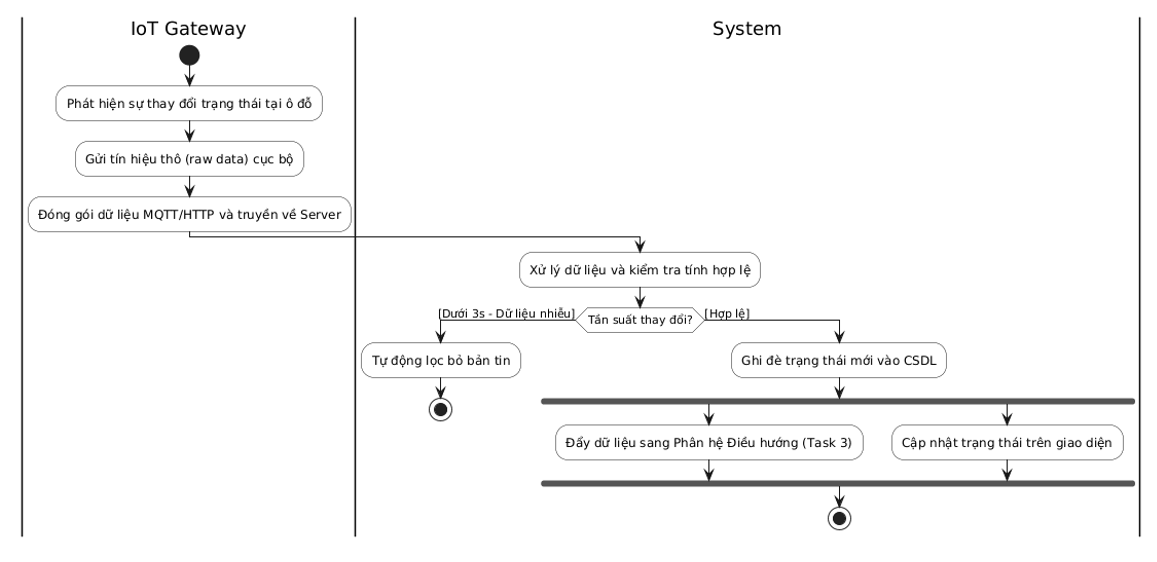
\includegraphics[width=0.8\textwidth]{pictures/act_diagram/ac_2.png} 
    \caption{Activity Diagram cho use-case Tự động cập nhật trạng thái ô đỗ}
    
\end{figure}

\newpage
\noindent \textbf{Giám sát kết nối và Cô lập thiết lỗi}
\begin{figure}[H]
    \centering
    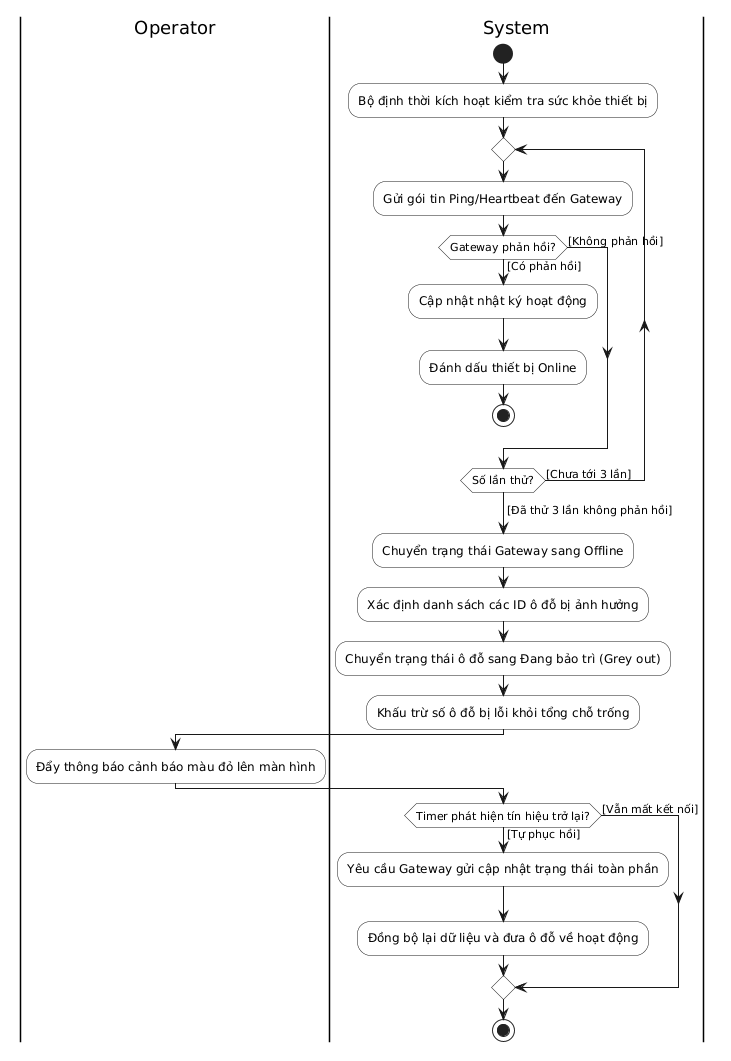
\includegraphics[width=0.8\textwidth]{pictures/act_diagram/ac_34.png} 
    \caption{Activity Diagram cho use-case Giám sát kết nối và Cô lập thiết lỗi}
   
\end{figure}